% for notes environment
\usepackage{xsavebox}

\usepackage{luatexja}
\usepackage[hiragino-pron, nfssonly, deluxe, expert]{luatexja-preset}
\usepackage{fontspec}
\usepackage{epigraph}
\usepackage{etoolbox}
\usepackage{tikz}
\usepackage{framed}
\usepackage{mathtools}
\usepackage{listings}
\usepackage{libertine}
\usepackage[libertine]{newtxmath}
\usepackage{bxcoloremoji}
\usepackage{xcolor}
\usepackage{diagbox}
\usepackage{caption}
\usepackage{appendixnumberbeamer}
\usepackage{todonotes}

\usetikzlibrary{fit}

\setmonofont{CMU Typewriter Text}

\definecolor{links}{HTML}{2A1B81}
\hypersetup{colorlinks,linkcolor=,urlcolor=links}

\usetheme{Boadilla}
\usecolortheme{seahorse}
% \usefonttheme{serif}

\setbeamercolor{page number in head/foot}{bg=blue!10}
\setbeamertemplate{footline}{%
  \leavevmode%
  \hbox{%
    \begin{beamercolorbox}[wd=.35\paperwidth,ht=2.25ex,dp=1ex,center]{author in head/foot}%
      \usebeamerfont{author in head/foot}\insertshortauthor\hspace*{1ex}(\insertshortinstitute)
    \end{beamercolorbox}%
    \begin{beamercolorbox}[wd=.3\paperwidth,ht=2.25ex,dp=1ex,center]{title in head/foot}%
      \usebeamerfont{title in head/foot}\insertshorttitle
    \end{beamercolorbox}%
    \begin{beamercolorbox}[wd=.25\paperwidth,ht=2.25ex,dp=1ex,center]{date in head/foot}%
      \insertshortdate{} @ \InsertConference
    \end{beamercolorbox}%
    \begin{beamercolorbox}[wd=.1\paperwidth,ht=2.25ex,dp=1ex,center]{page number in head/foot}%
      \insertframenumber{} / \inserttotalframenumber\hspace*{1ex}
    \end{beamercolorbox}}%
  \vskip0pt%
}

\beamertemplatenavigationsymbolsempty

\setbeamertemplate{bibliography item}{\insertbiblabel}
\setbeamersize{description width=1cm}
\setbeamertemplate{items}[circle]
\setbeamertemplate{section in toc}[circle]
\setbeamertemplate{subsection in toc}{%
  \leavevmode\leftskip=2em
  {%
    \usebeamerfont*{itemize item}%
    \usebeamercolor{subsection number projected}%
    \color{bg}%
    \raise1.25pt\hbox{\donotcoloroutermaths$\bullet$}}%
  \hskip1.5ex\inserttocsubsection\par}

% Definitions for the title page
\newcommand*{\GitHub}[1]{%
  \gdef\InsertGitHub{#1}%
}
\newcommand*{\Email}[1]{%
  \gdef\InsertEmail{\href{mailto:#1}{#1}}%
}
\newcommand*{\Conference}[1]{%
  \gdef\InsertConference{#1}%
}
\setbeamerfont{title}{size=\huge, series=\bfseries, family=\mcfamily\rmfamily}
\setbeamercolor{title}{bg=white}
\setbeamerfont{email}{size=\scriptsize, family=\ttfamily}
\setbeamercolor{email}{bg=white}
\setbeamerfont{date}{shape=\itshape, family=\rmfamily}
\setbeamerfont{vc}{size=\scriptsize, family=\ttfamily}
\setbeamercolor{vc}{bg=white}

\input{vc.tex}

\setbeamertemplate{title page}
{%
  \vbox{}
  \vfill
  \begingroup
    \centering
    \hrulefill
    \vskip0.5ex\par
    \begin{beamercolorbox}[sep=8pt,center,shadow=false,rounded=true]{title}
      \usebeamerfont{title}\inserttitle\par%
      \ifx\insertsubtitle\@empty%
      \else%
        \vskip0.25em%
        {\usebeamerfont{subtitle}\usebeamercolor[fg]{subtitle}\insertsubtitle\par}%
      \fi%     
    \end{beamercolorbox}%
    \hrulefill
    \vskip0.5ex\par
    \begin{beamercolorbox}[sep=0pt,center,shadow=false,rounded=true]{author}
      \usebeamerfont{author}\insertauthor
    \end{beamercolorbox}
    \begin{beamercolorbox}[sep=0pt,center,shadow=false,rounded=true]{email}
      \usebeamerfont{email}\InsertEmail
    \end{beamercolorbox}
    \vskip0.1ex
    \begin{beamercolorbox}[sep=5pt,center,shadow=false,rounded=true]{institute}
      \usebeamerfont{institute}\insertinstitute
    \end{beamercolorbox}
    \begin{beamercolorbox}[sep=5pt,center,shadow=false,rounded=true]{date}
      \usebeamerfont{date}\insertdate @ \InsertConference
    \end{beamercolorbox}
    \begin{beamercolorbox}[sep=0pt,center,shadow=false,rounded=true]{vc}
      \usebeamerfont{vc}
      \url{https://github.com/\InsertGitHub} (\texttt{\GITAbrHash})
    \end{beamercolorbox}
    % {\centering
    %   \href{https://creativecommons.org/licenses/by-nc/4.0/}{%
    %     
\includegraphics[width=0.1\textwidth]{img/by-nc.pdf}%
    %   }%
    % }
    {\usebeamercolor[fg]{titlegraphic}\inserttitlegraphic\par}
  \endgroup
  \vfill
}
\setbeamertemplate{blocks}[rounded][shadow=false]

% ============ ここを消すとNote消える ================
\mode<handout>{%
  \usepackage{pgfpages}
  \setbeameroption{show notes on second screen=right}
  \setbeamertemplate{note page}{%
    \vspace{2ex}\insertnote%
  }
}
% ============ ここを消すとNote消える ================


\renewcommand{\kanjifamilydefault}{\gtdefault}

\resetcounteronoverlays{lstlisting}
\definecolor{bluegray}{rgb}{0.4, 0.6, 0.8}
\DeclareCaptionFormat{listing}{{\color{bluegray}\lstlistingname}#2#3}
\captionsetup[lstlisting]{format=listing, font={footnotesize}}

\setmonofont[Ligatures=TeX]{CMU Typewriter Text}

\setbeamertemplate{items}[circle]

\newfontfamily\quotefont[Ligatures=TeX]{Linux Libertine O} % selects Libertine as the quote font

\newcommand*\quotesize{60} % if quote size changes, need a way to make shifts relative
% Make commands for the quotes
\newcommand*{\openquote}
   {\tikz[remember picture,overlay,xshift=0em,yshift=-3ex]
   \node (OQ) {\quotefont\fontsize{\quotesize}{\quotesize}\selectfont``};\kern0pt}

\newcommand*{\closequote}[1]
  {\tikz[remember picture,overlay,xshift=1ex,yshift={#1}]
   \node (CQ) {\quotefont\fontsize{\quotesize}{\quotesize}\selectfont''};}

\newcommand*\shadedauthorformat{\emph} % define format for the author argument

% Now a command to allow left, right and centre alignment of the author
\newcommand*\authoralign[1]{%
  \if#1l
    \def\authorfill{}\def\quotefill{\hfill}
  \else
    \if#1r
      \def\authorfill{\hfill}\def\quotefill{}
    \else
      \if#1c
        \gdef\authorfill{\hfill}\def\quotefill{\hfill}
      \else\typeout{Invalid option}
      \fi
    \fi
  \fi}
% wrap everything in its own environment which takes one argument (author) and one optional argument
% specifying the alignment [l, r or c]
%
\newenvironment{shadequote}[2][l]%
{\authoralign{#1}
\ifblank{#2}
   {\def\shadequoteauthor{}\def\yshift{-2ex}\def\quotefill{\hfill}}
   {\def\shadequoteauthor{\par\authorfill\shadedauthorformat{#2}}\def\yshift{2ex}}
\begin{quote}\normalfont\openquote}
{\shadequoteauthor\quotefill\closequote{\yshift}\end{quote}}

\makeatletter
\def\@fnsymbol#1{\ensuremath{\ifcase#1\or *\or \dagger\or \ddagger\or
   \mathsection\or \mathparagraph\or \|\or **\or \dagger\dagger
   \or \ddagger\ddagger \else\@ctrerr\fi}}
\makeatother

\renewcommand{\thefootnote}{\fnsymbol{footnote}}

\newcommand\ballcircle[1]{%
  {%
    \usebeamercolor{enumerate item}%
    \tikzset{beameritem/.style={circle,inner sep=0,minimum size=2ex,text=enumerate item.bg,fill=enumerate item.fg,font=\footnotesize}}%
    \tikz[baseline=(n.base)]\node(n)[beameritem]{\sffamily#1};%
  }%
}
\newcommand\ballref[1]{%
  \ballcircle{\ref{#1}}%
}

\usetikzlibrary{calc}
\usetikzlibrary{shapes.callouts} 

\pgfkeys{%
    /calloutquote/.cd,
    width/.code                   = {\def\calloutquotewidth{#1}},
    position/.code                = {\def\calloutquotepos{#1}}, 
    author/.code                  = {\def\calloutquoteauthor{#1}},
    at/.code                      = {\def\calloutquoteat{#1}},
    sign/.code                    = {\def\calloutquotesign{#1}},
    /calloutquote/.unknown/.code  = {\let\searchname=\pgfkeyscurrentname
                                      \pgfkeysalso{\searchname/.try=#1,                        
                                      /tikz/\searchname/.retry=#1},\pgfkeysalso{\searchname/.try=#1,
                                      /pgf/\searchname/.retry=#1}
                                    }
}

\makeatletter

\newsavebox\temp@simple@callout@author@box
\newcommand\calloutquote[2][]{%
  \pgfkeys{/calloutquote/.cd,
    width    = 5cm,
    position = {(0.5,-0.2)},
    at       = {(0,0)},
    author   = {},
    sign     = {+}
  }%
  \pgfqkeys{/calloutquote}{#1}%
  \sbox{\temp@simple@callout@author@box}{\mbox{%
    \begin{tabular}{l}
      \calloutquoteauthor%
    \end{tabular}
  }}%
  \node [rectangle callout,callout relative pointer={\calloutquotepos},align=center,text width=\calloutquotewidth,/calloutquote/.cd,
     #1] (tmpcall) at \calloutquoteat {#2};
  \node at ($ (tmpcall.pointer) - (-\calloutquotesign0.5\wd\temp@simple@callout@author@box,0.7\ht\temp@simple@callout@author@box) $) {\calloutquoteauthor};
}

\newsavebox\temp@simple@callout@box
\newcommand{\simplecallout}[4][{}]{%
  \sbox{\temp@simple@callout@box}{\mbox{%
    \begin{tabular}{l}
      #4%
    \end{tabular}
  }}%
  \begin{center}%
    \begin{tikzpicture}%
      \calloutquote[width=1.05\wd\temp@simple@callout@box,position={(#2.5,-0.2)},fill=#3,rounded corners,author={#1},sign=#2]{
        #4%
      }%
    \end{tikzpicture}%
  \end{center}
}

\makeatother
\newfontfamily{\listingfont}[Scale=0.85]{Menlo}
\definecolor{dkgreen}{rgb}{0,0.6,0}
\definecolor{gray}{rgb}{0.5,0.5,0.5}
\definecolor{mauve}{rgb}{0.58,0,0.82}

\makeatletter
\lst@CCPutMacro\lst@ProcessOther {"2D}{\lst@ttfamily{-{}}{-{}}}
\@empty\z@\@empty
\makeatother

\lstdefinestyle{csharp}{
  numbers=left,
  language=[Sharp]C
}

\lstdefinestyle{cil}{
  numbers=left,
  language=CIL
}

\lstdefinestyle{plain}{
  basicstyle=\listingfont\tiny,
  language=
}

\lstdefinestyle{sh}{
  numbers=left,
  language=sh
}

\lstdefinestyle{c}{
  numbers=left,
  language=C
}

\lstdefinestyle{python}{
  numbers=left,
  language=Python
}

\lstdefinestyle{asm-x86}{
  numbers=left
}

\lstdefinestyle{pseudo-code}{
  numbers=left,
  keywords=[6]{for,from,to,endfor,while,endwhile}
}

\lstdefinestyle{bitcoin-script}{
  mathescape=true
}

\lstset{
  basicstyle=\listingfont,
  frame=single,
  xleftmargin=2em,
  xrightmargin=1em,
  breaklines=true
}

\lstdefinestyle{scala}{
  basicstyle=\listingfont\scriptsize,
  breakatwhitespace=false,
  language=scala,
  captionpos=b,
  commentstyle=\listingfont\scriptsize\color{dkgreen},
  extendedchars=true,
  xleftmargin=1em,
  xrightmargin=1em,
  keepspaces=true,
  keywordstyle=\listingfont\scriptsize\color{blue},
  emphstyle=\listingfont\scriptsize\color{cyan},
  rulecolor=\listingfont\scriptsize\color{black},
  showspaces=false,
  showstringspaces=false,
  showtabs=false,
  stringstyle=\listingfont\scriptsize\color{mauve},
  tabsize=2
}

\lstdefinelanguage{scala}{
  morekeywords={abstract,case,catch,class,def,%
    do,else,extends,false,final,finally,%
    for,if,implicit,import,match,mixin,%
    new,null,object,override,package,%
    private,protected,requires,return,sealed,%
    super,this,throw,trait,true,try,%
    type,val,var,while,with,yield},
  moreemph={Byte,Short,Int,Long,Float,Double,Char,
    String,Boolean,Unit,Null,Nothing,Any,AnyRef,
    Left,Right,Either},
  otherkeywords={=>,<-,<\%,<:,>:,\#,@},
  sensitive=true,
  morecomment=[l]{//},
  morecomment=[n]{/*}{*/},
  morestring=[b]",
  morestring=[b]',
  morestring=[b]"""
}

\lstdefinestyle{go}{
  basicstyle=\listingfont\scriptsize,
  breakatwhitespace=false,
  language=go,
  captionpos=b,
  commentstyle=\listingfont\scriptsize\color{dkgreen},
  extendedchars=true,
  xleftmargin=1em,
  xrightmargin=1em,
  keepspaces=true,
  keywordstyle=\listingfont\scriptsize\color{blue},
  emphstyle=\listingfont\scriptsize\color{cyan},
  rulecolor=\listingfont\scriptsize\color{black},
  showspaces=false,
  showstringspaces=false,
  showtabs=false,
  stringstyle=\listingfont\scriptsize\color{mauve},
  tabsize=2
}


\lstdefinelanguage{golang}%
  {morekeywords=[1]{package,import,func,type,struct,return,defer,panic,%
     recover,select,var,const,iota},%
   morekeywords=[2]{string,uint,uint8,uint16,uint32,uint64,int,int8,int16,%
     int32,int64,bool,float32,float64,complex64,complex128,byte,rune,uintptr,%
     error,interface},%
   morekeywords=[3]{map,slice,make,new,nil,len,cap,copy,close,true,false,%
     delete,append,real,imag,complex,chan,},%
   morekeywords=[4]{for,break,continue,range,go,goto,switch,case,fallthrough,if,%
     else,default,},%
   morekeywords=[5]{Println,Printf,Error,Print,},%
   sensitive=true,%
   morecomment=[l]{//},%
   morecomment=[s]{/*}{*/},%
   morestring=[b]',%
   morestring=[b]",%
   morestring=[s]{`}{`},%
}
\newenvironment{notes}
  {%
    \begin{xlrbox}{NotesBox}
    \begin{minipage}{.95\textwidth}
    \small\rmfamily\mcfamily
    \begin{itemize}
    \setlength{\itemindent}{0em}
    \setlength{\footnotesep}{5mm}
  }{%
    \end{itemize}
    \end{minipage}
    \end{xlrbox}
    \note{\theNotesBox}}

\def\AtSOne#1\csod{%
	\begin{array}{c|}
		\hline
		#1\\
		\hline
	\end{array}
}%
\def\AtSTwo#1,#2\csod{%
	\begin{array}{c|c|}
		\hline
		#1 & #2\\
		\hline
	\end{array}
}%
\def\AtSThree#1,#2,#3\csod{%
	\begin{array}{c|c|c|}
		\hline
		#1 & #2 & #3\\
		\hline
	\end{array}
}%
\def\AtSFour#1,#2,#3,#4\csod{%
	\begin{array}{c|c|c|c|}
		\hline
		#1 & #2 & #3 & #4\\
		\hline
	\end{array}
}%
\def\AtSFive#1,#2,#3,#4,#5\csod{%
	\begin{array}{c|c|c|c|c|}
		\hline
		#1 & #2 & #3 & #4 & #5\\
		\hline
	\end{array}
}%
\def\AtSSix#1,#2,#3,#4,#5,#6\csod{%
	\begin{array}{c|c|c|c|c|c|}
		\hline
		#1 & #2 & #3 & #4 & #5 & #6\\
		\hline
	\end{array}
}
\newcommand{\SOne}[1]{\AtSOne#1\csod}
\newcommand{\STwo}[1]{\AtSTwo#1\csod}
\newcommand{\SThree}[1]{\AtSThree#1\csod}
\newcommand{\SFour}[1]{\AtSFour#1\csod}
\newcommand{\SFive}[1]{\AtSFive#1\csod}
\newcommand{\SSix}[1]{\AtSSix#1\csod}

\newcommand\ce[1]{%
  \coloremojiucs{#1}
}

\presetkeys{todonotes}{inline, noinlinepar}{}

\title[An interpreter handling over effects for Eff]{%
  An interpreter handling \\
  over effects for Eff%
}
\author[Yoshimura Hikaru]{%
  \textsc{Yoshimura} Hikaru(吉村 優)
}
\Email{hikaru\_yoshimura@r.recruit.co.jp}
\date[October 17, 2020]{%
  \oldstylenums{October 17, 2020}
}
\Conference{ScalaMatsuri 2020}
\institute[\InsertEmail]{%
  Recruit Marketing Partners Co., Ltd.
}
\GitHub{y-yu/scalamatsuri2020}

\begin{document}

\setlength{\leftmargini}{1em}

\begin{frame}
  \maketitle

  \note{%
    \vspace*{\fill}
    \centering
    {\LARGE エフェクトを跨ぐインタープリター}
    \vspace{2ex}
    
    \begin{itemize}
      \item こっちのページは日本語の説明となります。
      
      \item 翻訳の方向けの情報もはいっているので、多少は冗長かもしれないです。
    \end{itemize}
    \vspace*{\fill}
  }%
\end{frame}

\begin{frame}
  \frametitle{Table of contents}

  \tableofcontents

  \begin{notes}
    \item このトークでは、まずモナドよりも前の
    低レイヤーな方法を紹介しつつ、それの問題と
    これまでどういう方法で解決してきたか?ということを通して
    モナドなどについて解説する。
    そのあとEffとインタープリターの説明をして
    最後にこのトークのテーマである「エフェクトを跨ぐインタープリター」を実装する。
  \end{notes}
\end{frame}

\section{Who am I?}
\begin{frame}
  \frametitle{Who am I?}
  
  \begin{columns}
    \begin{column}{0.3\textwidth}
      \begin{center}
        \begin{figure}[h]
          
\includegraphics[width=0.95\textwidth]{img/bird2x.png}%
        \end{figure}
      \end{center}
 
      \begin{table}[h]
        \begin{tabular}{ll}
          Twitter & \href{https://twitter.com/\_yyu\_}{@\_yyu\_} \\
          Qiita &  \href{https://qiita.com/yyu}{yyu} \\
          GitHub &  \href{https://github.com/y-yu}{y-yu} \\
          % Facebook & \href{https://www.facebook.com/h1karuy}{h1karuy} \\
        \end{tabular}
      \end{table}
    \end{column}
    \begin{column}{0.7\textwidth}
      \pause
      \begin{itemize}
        \item Recruit Marketing Partners Co., Ltd.
        \begin{itemize}
          \item StudySapuri ENGLISH server side(Scala)
        \end{itemize}

        \item Quantum Information
        \begin{itemize}
          \item but I don't know well about Quantum annealing...
        \end{itemize}

        \item Cryptography \& Security
        
        \item {\LaTeX} typesetting
      \end{itemize}
    \end{column}
  \end{columns}

  \begin{notes}
    \item リクルートマーケティングパートナーズに中途入社した。
    \item スタディサプリENLGISHのサーバーサイドをScalaで作っている。
    \item 量子コンピューター(\emph{Quantum Information})%
    \footnote{ふつう量子コンピューターは``Quantum Computer''となるが、%
      Quantum Computerであると物理的なハードウェアなニュアンスもあるため、
      そうではなくて量子コンピューター上で動作する(予定の)ソフトウェアまたは
      プロトコルを意図して量子情報(``Quantum Information'')とした。
      (必要ないかも\ce{:thinking:})}
    についても興味がある。

    \item 暗号やセキュリティーについても好きで、今も少しはCTF\footnote{``Capture The Flag''、セキュリティー系の競技のこと。}%
    に出場したりもする。

    \item 最後にこのスライドを作るのにも使った{\LaTeX}も非常に好きで、実はScala以上に利用歴がある。
    
  \end{notes}
\end{frame}


\section{Introduction}

\begin{frame}
  \frametitle{Concrete case I'll talk about}

  \pause
  \simplecallout[{
\includegraphics[width=0.2\textwidth]{./img/seminar.png}}]{+}{cyan!10}{In this talk, we think about one concrete case:}

  \pause
  \begin{shadequote}{}
    \begin{center}
      \itshape\rmfamily\Large
      Read \& Write data to database with the transaction
    \end{center}
  \end{shadequote}

  \begin{itemize}
    \item<+-> This is very common case in the programming, but there are many ways to do it
  \end{itemize}

  \begin{notes}
    \item このトークでは、全体を通して1つの具体的なケースである、
    ``データベースにトランザクションを張りながら読み書きをする''という話を例にする。

    \item プログラミングにおいて、これはかなりありふれたケースだが、
    いろいろなやり方がある。

    \item 低レベルなやり方やそれの問題を述べつつ、最終的にそういった問題が
    \lstinline|Eff|でどう解決されるのか?について説明していく。
  \end{notes}
\end{frame}

\section{Low Level Example}

\begin{frame}[fragile]
  \frametitle{Low level example}

  \begin{columns}
    \begin{column}{0.5\textwidth}
      \pause
\begin{lstlisting}[style=scala]
val transactionManager = new TM()
val session = transactionManager.begin()

databaseOperation(
  // If you want to rollback,
  // call `session.fail`
  session
)

if (transactionManager.commit(session))
  /* Successful */
else
  /* Failure */   
\end{lstlisting}
    \end{column}
    \begin{column}{0.5\textwidth}

      \pause
      \begin{itemize}
        \item<+-> It's (maybe) used in tranditional languages like C
       
        \item<+-> You know, that way has some problems:
      \end{itemize}
    \end{column}
  \end{columns}


  \uncover<+->{%
    \simplecallout[\huge\ce{:thinking:}]{+}{red!10}{Could programmers \emph{forget} to write \lstinline|begin| and \lstinline|commit|?}%
  }

  \begin{notes}
    \item まず念のために言うとしたら、低レベルというのが常に悪いということではない。

    \item ただ考えないといけないことが増えたり、考え忘れたりするとひどいことになりやすい。
    考え忘れるというのがどういうことなのか?それを具体的にみていく。

    \item 今このようなコードでトランザクションをかけながらDBへのアクセスをする。

    \item \lstinline|TM|は``トランザクションマネージャー''のことで、
    これがDBのトランザクションを管理して、\lstinline|begin|・\lstinline|commit|で
    トランザクションの開始・終了を表す。

    \item 冒頭に言った「考えわすれる」というのは、このコードで言えば
    \lstinline|begin|・\lstinline|commit|を忘れるということ。
  \end{notes}
\end{frame}


\begin{frame}[fragile]
  \frametitle{Loan pattern}

  \begin{itemize}
    \item If the problem is forgetting,
    we can use \emph{Loan pattern}:
  \end{itemize}

  \begin{columns}
    \begin{column}{0.52\textwidth}
\begin{lstlisting}[style=scala]
def withTransaction(
  f: Session => A
): Either[Throwable, A] = {
  val session = transactionManager.begin()
  val a = f(session)
  if (transactionManager.commit(session)) Right(a)
  else Left(new RuntimeException())
}

withTransaction { session =>
  something.databaseOperation(session)
}
\end{lstlisting}
    \end{column}
    \begin{column}{0.48\textwidth}

      \pause
      \begin{itemize}
        \setlength{\itemindent}{0em}
        \item<+-> \lstinline|withTransaction| takes a function \lstinline|f|

        \item<+-> And then execute it inside the \lstinline|begin| and \lstinline|commit|
      \end{itemize}

      \uncover<+->{%
        \simplecallout[{
\includegraphics[width=0.2\textwidth]{./img/hacker_white.png}}]{-}{blue!10}{%
          Is Loan pattern the silver bullet?%
        }
      }
    \end{column}
  \end{columns}
  \begin{notes}
    \item この「忘れる」問題への対処として``ローンパターン''が知られている。

    \item このように関数を取る関数\lstinline|withTransaction|に関数\lstinline|f|を
    渡してそれをトランザクション内で実行する

    \item こうすればデータベースのトランザクションのように「借りたもの(Loan)」を
    返し忘れることがない%
    \footnote{トランザクションを著者が完全に理解しているわけでもないが、%
    データベースの一貫性などを担保する目的で一時的に利用するものであって、永遠に%
    利用することはできないので、いずれは返す(解放する)必要があるということを言いたい。}。

    \item こうすれば少なくとも忘れる問題には対処できるが、
    はたしてこれだけでOKだろうか?
  \end{notes}
\end{frame}

\begin{frame}[fragile]
  \frametitle{Nested loan pattern}

  \pause
  \begin{itemize}
    \item<+-> We can use \lstinline|withTransaction| \emph{illegally} like below
  \end{itemize}

  \begin{columns}
    \begin{column}{0.5\textwidth}
\begin{lstlisting}[style=scala]
def ops(): Either[Throwable, ?] =
  withTransaction { session =>
    something.databaseOperation(session)
  }

withTransaction { session =>
  /* something using session */
  ops()
}
\end{lstlisting}
    \end{column}
    \begin{column}{0.5\textwidth}
      \simplecallout[{
\includegraphics[width=0.15\textwidth]{./img/hacker_laugh}}]{+}{orange!10}{%
        Use \lstinline|withTransaction| in \\
        the other \lstinline|withTransaction| \ce{:smiling_imp:}
      }
    \end{column}
  \end{columns}

  \begin{itemize}
    \item<+-> No one wants to do that but it's allowed...\ce{:innocent:}

    \item<+-> Indeed, we don't actually ``forget'' to write \lstinline|begin| and \lstinline|commit|,
    but the other problem remains
    \begin{itemize}
      \item In addtion, the first low level example \textbf{also} has this problem
    \end{itemize}
  \end{itemize}

  \begin{notes}
    \item ただLoan patternはこのように無理やり入れ子にして使うこともできてしまう……。

    \item こうやって使いたい人は恐らく誰もいないが、しかし型システム(\emph{type system})上は
    このようなコードが許可されてしまう。

    \item たしかに忘れるということは防げるものの、問題は他にも残っている。

    \item ただ、この入れ子になってしまう問題は一番最初に紹介した低レベルの方法でも起きることであって、
    Loan patternはそれよりは少なくとも安全にはなっているはずである。
  \end{notes}
\end{frame}

\section{Monad and Monad Transformer}

\begin{frame}[fragile]
  \frametitle{Monad}

  \pause
  \begin{itemize}
    \item We can use \lstinline|map| and \lstinline|flatMap|
    instead of raw Loan pattern
  \end{itemize}

  \begin{columns}
    \pause
    \begin{column}{0.55\textwidth}
\begin{lstlisting}[style=scala]
case class DBIO[A](
  run: Session => A 
) {
  def map[B](f: A => B): DBIO[B] =
    flatMap(a => DBIO(_ => f(a)))

  def flatMap[B](f: A => DBIO[B]): DBIO[B] =
    DBIO(s => f(run(s)).run(s))
}
\end{lstlisting}
    \end{column}
    \pause
    \begin{column}{0.45\textwidth}
      \begin{itemize}
        \item And define this utility function: \lstinline|ask|
      \end{itemize}

\begin{lstlisting}[style=scala]
object DBIO {
  def ask: DBIO[Session] =
    DBIO(s => s)
}
\end{lstlisting}
    \end{column}
  \end{columns}

  \pause
  \begin{itemize}
    \item We can implement code that access to the database
    with \lstinline|DBIO|
  \end{itemize}

\begin{lstlisting}[style=scala]
def greatDBOps1: DBIO[?] =
  DBIO.ask map { session: Session =>
    session.execute(/* Great Operation! */)
  }
\end{lstlisting}

  \begin{notes}
    \item そこでLoan patternを生で使うのではなくて、
    \lstinline|map|と\lstinline|flatMap|でラップ(wrap)する。

    \item このように\lstinline|DBIO|\footnote{\emph{Database Input/Output}の略。}%
    というデータ構造をつくって、
    それに\lstinline|map|・\lstinline|flatMap|を実装する。

    \item さらにユーティリティーとして\lstinline|ask|というのを
    このように作っておく。

    \item そうすればDBにアクセスするようなコードを\lstinline|ask|で
    こうやって書くことができる。
  \end{notes}
\end{frame}

\begin{frame}[fragile]
  \frametitle{Monad}

  \begin{columns}
    \begin{column}{0.6\textwidth}
      \begin{itemize}
         \item \lstinline|greatDBOps1|, \lstinline|greatDBOps2| and \lstinline|greatDBOps3|
         run in the same transaction\ce{:laughing:}
      \end{itemize}

      \uncover<.(2)->{%
        \simplecallout[{
\includegraphics[width=0.2\textwidth]{./img/computer_man.png}}]{-}{blue!10}{%
          Is there \emph{well-known monad} \\
          which can do the same things?
        }%
      }
    \end{column}
    \begin{column}{0.4\textwidth}
\begin{lstlisting}[style=scala]
val dbio: DBIO[Int] = for {
  a <- greatDBOps1
  b <- greatDBOps2
  c <- greatDBOps3(a, b)
} yield c

withTransaction { session =>
  dbio.run(session)
}
\end{lstlisting}
    \end{column}
  \end{columns}

  \pause
  \begin{itemize}
    \item<.(2)-> Yes, \lstinline|DBIO[A]| is the same as \lstinline|Reader[Session, A]|
  \end{itemize}

  \begin{notes}
    \item あとは1つのトランザクションに入れたいコードを\lstinline|for|で合成(composition)
    していけばいい。

    \item 最後に\lstinline|DBIO|の\lstinline|run|をLoan pattern用の関数
    \lstinline|withTransaction|の中で実行してやればいい。

    \item もちろん\lstinline|DBIO|の中で\lstinline|withTransaction|することもできるが、
    型として``DBにアクセスする操作の型は\lstinline|DBIO|である''となっているので、
    これを入れ子にしてしまうことは多少防がれるはずである。

    \item ところで\lstinline|DBIO|は新規で作ったが、同じことができる
    よく知られたモナドがあるのではないだろうか?

    \item それは正解で\lstinline|DBIO[A]|は環境(\emph{environment})を
    \lstinline|Session|に固定したReaderモナドである
    \lstinline|Reader[Session, A]|と同じような感じである。
  \end{notes}
\end{frame}

\begin{frame}
  \frametitle{Next step}

  \pause
  \begin{itemize}
    \item \lstinline|DBIO| represents \emph{just} a Database I/O
    \begin{itemize}
      \item but we sometimes want to use other (side) effects...
    \end{itemize}
  \end{itemize}

  \pause
  \simplecallout[\huge\ce{:thinking:}]{+}{red!10}{%
    What are the other side effects?
  }

  \pause
  \begin{itemize}
    \item It's time to go to the next step:
  \end{itemize}
  
  \begin{shadequote}{}
    \begin{center}
      \itshape\rmfamily\large
      We want to send e-mails only if the database transaction
      is successful
    \end{center}
  \end{shadequote}

  \begin{notes}
    \item \lstinline|DBIO|はデータベースI/Oというただ1つを表現するが、
    他の副作用を利用したいときもある。

    \item そこで次は、データベーストランザクションが成功したときに
    メールを送信するというシチュエーションを考えていく。
  \end{notes}
\end{frame}

\begin{frame}
  \frametitle{Email}

  \begin{flushright}
    
\includegraphics[width=0.2\textwidth]{./img/computer_mail.png}
  \end{flushright}

  \pause
  \begin{itemize}
    \item<+-> Sending e-mail is as popular as using database

    \item<+-> Database has transactions but e-mail \emph{doesn't}

    \item<+-> So we want to send e-mail after all operations
    are done successfully
  \end{itemize}

  \begin{notes}
    \item メールを送るというのもまた、データベースを使ったプログラミングと同じくらい
    よくある処理である。

    \item 必要ないかもしれないが、

    \item データベースとの大きな違いとして、メールの送信にトランザクションは
    \textbf{存在しない}。あたりまえのことだが、メールを送った後に後続の処理が
    失敗したとしても、いったん送信してしまったメールを取り消すことはできない。

    \item したがってメールの送信は全ての処理が正常に終了となったあとに行いたい。
  \end{notes}
\end{frame}

\begin{frame}[fragile]
  \label{fra:send_email_definition}
  \frametitle{Naive approach}

  \begin{columns}
    \pause
    \begin{column}{0.5\textwidth}
      \begin{itemize}
        \item There is a sending e-mail function that has
        such an interface:
\begin{lstlisting}[style=scala]
def sendMail(
  mail: Mail
): Either[Throwable, Unit]
\end{lstlisting}

        \begin{itemize}  
          \item \lstinline|Mail| consists of to-address,
          from-address, title and email body
        \end{itemize}
      \end{itemize}
    \end{column}

    \pause
    \begin{column}{0.5\textwidth}
      \begin{itemize}
        \item And then we use this after the database transaction
      \end{itemize}

\begin{lstlisting}[style=scala]
val result = withTransaction { session =>
  dbio.run(session)
}

if (result.isRight)
  sendMail(greatEmail) match {
    case Left(e) => /* something */
    case _       => ()
  }
\end{lstlisting}
    \end{column}
  \end{columns}

  \pause
  \simplecallout[{
\includegraphics[width=0.1\textwidth]{./img/computer_man.png}}]{-}{cyan!10}{%
    The \emph{code distance} between \lstinline|sendMail| and DB operation is too far away
  }

  \begin{notes}
    \item まずメールを送る関数\lstinline|sendMain|を次のように定義する。
    成功したら\lstinline|Either.Right|で失敗したら\lstinline|Left|となる。
     
    \item さて、一番ナイーブにはこのように\lstinline|withTransaction|
    の後でDBセッションの状態をチェックしつつ実行すればよい。
     
    \item 動きそうだが、これはちょっと\lstinline|sendMain|と
    データベース処理の間のコード上の距離が離れすぎてないか……?
  \end{notes}
\end{frame}
 
\begin{frame}[fragile]
  \frametitle{Cohesion}

  \begin{columns}
    \begin{column}{0.5\textwidth}
      \simplecallout{+}{green!10}{%
        What is the code distance?
      }
    \end{column}
    \begin{column}{0.5\textwidth}
      \simplecallout{-}{blue!10}{%
        It's known as \emph{cohesion}
      }
    \end{column}
  \end{columns}

  \pause
  \begin{itemize}
    \item We implement the DB operating function that returns \lstinline|DBIO|

\begin{lstlisting}[style=scala]
def userUpdate(newUserInfo: UserInfo): DBIO[Unit] =
  DBIO.ask map { session =>
    /* Great user update logic is here!!!! */
  }
\end{lstlisting}
  \end{itemize}

  \pause
  \simplecallout[\LARGE\ce{:rage:}]{+}{red!10}{%
    We want to write sending e-mail logic here too!
  }

  \pause
  \begin{itemize}
    \item But actually we can only write e-mail logic
    behind the \lstinline|withTransaction| \ce{:innocent:}
    \begin{itemize}
      \item It means that our code is low cohesion
    \end{itemize}
  \end{itemize}

  \begin{notes}
    \item コードの距離とはどういうことか?ようするに凝集度(\emph{cohesion})のこと。

    \item \lstinline|DBIO|を使った関数を書くが、
    この場所にメールの送信処理を書くことはできない。

    \item しかしユーザーの変更処理はメールを送信することも1つのビジネスロジックであるから、
    DDD的にどこでやるか?などはいったん放置するにしてもビジネスロジックの近辺に
    あった方が凝集度が高くなりそうだ。

    \item でも我々の今の方法では\lstinline|withTransaction|のところに
    書かざるを得ない……
  \end{notes}
\end{frame}

\begin{frame}[fragile]
  \frametitle{Cohesion}

  \simplecallout[{
\includegraphics[width=0.1\textwidth]{./img/computer_man.png}}]{-}{cyan!10}{%
    OK. How about to return \lstinline|DBIO[Either[Throwable, A]]|?
  }
   
  \begin{columns}
    \pause
    \begin{column}{0.6\textwidth}
\begin{lstlisting}[style=scala]
def userUpdate(
  newUserInfo: UserInfo
): DBIO[Either[Throwable, Unit]] =
  DBIO.ask map { session =>
    val result = /* Great user update logic */
    val mail = /* Great e-mail from newUserInfo */

    if (result)
      sendMail(greatEmail)
    else
      Left(/* error! */)
  }
\end{lstlisting}
    \end{column}
    \pause
    \begin{column}{0.4\textwidth}
      \begin{itemize}
        \item<+-> Is it OK?\ce{:thinking:}

        \item<+-> This code appears to have high cohesion, unlike before
      \end{itemize}
    \end{column}
  \end{columns}

  \begin{notes}
    \item そういう問題があるので、じゃあ\lstinline|DBIO[Either[Throwable, A]]|を使ったらどうか?

    \item これはコード例のように\lstinline|DBIO.ask.map|の中で\lstinline|Either|を返すようにする。
    このようにすれば、\lstinline|DBIO|を利用するところでメールの送信ロジックを記述できる。

    \item したがって凝集度は向上すると考えられるが、これでいいだろうか?
  \end{notes}
\end{frame}

\begin{frame}[fragile]
  \frametitle{Monad transformer}

  \simplecallout[{
\includegraphics[width=0.09\textwidth]{./img/hacker_white.png}}]{+}{green!10}{%
    We can use \emph{monad transformer} such as \lstinline|EitherT|
  }

  \pause
  \begin{itemize}
    \item Monad transformer takes a monadic type constructor
    and turns it into a monad
  \end{itemize}

  \begin{columns}
    \begin{column}{0.45\textwidth}
\begin{lstlisting}[style=scala]
def userUpdateT(
  newUserInfo: UserInfo
): EitherT[DBIO, Throwable, Unit] =
  userUpdate(newUserInfo).toEitherT
\end{lstlisting}
    \end{column}
    \begin{column}{0.55\textwidth}
      \begin{itemize}
        \item Scala's \lstinline|for| only can access
        the most outer monad

        \item So if we use \lstinline|EitherT| rather than \lstinline|Either|,
        it will be easy to access \lstinline|Either| monad
        inside \lstinline|DBIO|
      \end{itemize}
    \end{column}
  \end{columns}

  \begin{notes}
    \item いったんこのコードが意図した動作をするか?というところは放置して、
    このようにモナドトランスフォーマー(\emph{Monad transformer})を利用することもできる。

    \item モナドトランスフォーマーは、モナドとなる型を取って(\emph{take})
    モナドとなるような高階(\emph{higher kind})な型コンストラクターである。

    \item ここでは\lstinline|EitherT|の詳細を説明しないが、このように
    モナド\lstinline|DBIO|を引数にとって\lstinline|DBIO|と\lstinline|Either|の
    両方の能力を持つ新たなモナドとなる。

    \item Scalaの\lstinline|for|式(\emph{expression})一番外側のモナドにしか
    アクセスできないため、モナドトランスフォーマーを利用して1つにすると取り扱いしやすくなる。
  \end{notes}
\end{frame}

\begin{frame}[fragile]
  \frametitle{Email failure example}

  \pause
  \begin{itemize}
    \item You maybe know,
    both \lstinline|DBIO[Either[Throwable, A]]| and
    \lstinline|EitherT[DBIO, Throwable, A]| have such a problem:
  \end{itemize}
  
  \begin{columns}
    \begin{column}{0.6\textwidth}
      \simplecallout[{
\includegraphics[width=0.15\textwidth]{./img/hacker_laugh}}]{-}{cyan!10}{%
        The e-mail in \lstinline|userUpdate| will be sent \\
        even if \lstinline|maybeFail| fails
      }
    \end{column}
    \begin{column}{0.4\textwidth}
\begin{lstlisting}[style=scala, escapeinside={|*}{*}]
val dbio = for {
  // With sending e-mail here
  _ <- userUpdate(newUserInfo)
  _ <- maybeFail // |*\ce{:bomb:}\ce{:smiling_imp:}*
} yield ???

withTransaction(dbio.run)
\end{lstlisting}
    \end{column}
  \end{columns}

  \pause
  \simplecallout[\LARGE\ce{:rage:}]{+}{orange!10}{%
    It's no good that database I/O are rollbacked
    however e-mail has been sent!
  }
  
  \begin{notes}
    \item もうすでに気がついているかもしれないが、
    このように\lstinline|for|で合成したときに後続の
    処理の\lstinline|DBIO|で失敗したとしても、メールは送信されてしまう。

    \item \lstinline|DBIO|が失敗したということはデータベースは
    ロールバックで操作がすべてなかったこととなる。しかしメールは
    途中までの処理が成功した!という内容で送信される。

    \item したがってこれはメールとデータベースの間で
    \textbf{不整合}(\emph{inconsistency})が生じた状態であり、避けるべきである。
  \end{notes}
\end{frame}

\begin{frame}
  \frametitle{Summary up to this point}

  \pause
  \begin{itemize}
    \item<+-> We want \textbf{both} \emph{cohesion and consistency}

    \item<+-> Up to this point of my talk,
    there seems to be a trade-off between the two

    \item<+-> In my opinion, there are two ways to combine them:
    \begin{enumerate}
      \item \label{enum:make_original_monad}
      Make an original moand to do it

      \item \label{enum:use_eff}
      Use \lstinline|Eff| and implement its
      suitable \emph{interpreter} for the trade-off
    \end{enumerate}

    \item<+-> First, I will describe option \ballref{enum:use_eff}.
    Then I will present my opinion on which is the better choice
  \end{itemize}

  \begin{notes}
    \item ここまでのまとめをすると、凝集度と一貫性(\emph{consistency})を両立したいが、
    しかしここまでに紹介した技術では「どちらを取るか?」というトレードオフになる。

    \item 自分の知る限りで、この問題への対処方として2つの方法があり、
    \begin{enumerate}
      \item 専用のオリジナルモナドを作ってしまうこと

      \item \lstinline|Eff|と専用のインタープリターをつくること
    \end{enumerate}
    それがこの\ce{:point_up:}2つである。

    \item まずここから\ballcircle{2}の話しをしていき
    そのあとで自分の考えとして\ballcircle{1}と\ballcircle{2}で
    どちらがよいと思っているのか?を話すことにする。
  \end{notes}
\end{frame}

\section{Eff and Interpreter}

\begin{frame}
  \frametitle{Table of contents}
  \tableofcontents[currentsection]

  \begin{notes}
    \item ここまでで目次にあった\lstinline|Eff|以外の部分の説明が
    終わったので、ここからようやく\lstinline|Eff|の説明にはいっていく。
  \end{notes}
\end{frame}

\begin{frame}
  \frametitle{%
    What is Eff%
    \footnote[frame]{In this talk, \lstinline|Eff| is based on \href{https://github.com/atnos-org/eff}{\texttt{atnos-eff}}.}%
  }

  \pause
  \begin{itemize}
    \item<+-> \lstinline|Eff| is a type constructor which takes two types: \lstinline|R| and \lstinline|A|
    \begin{center}
      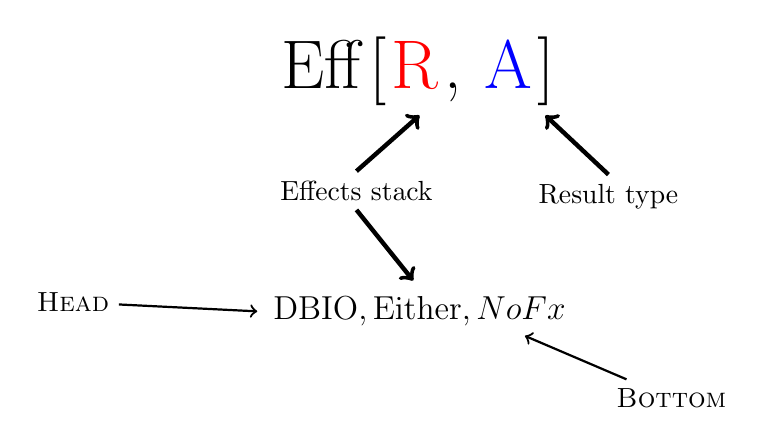
\begin{tikzpicture}[scale=0.8]
        \node (A) at (0, 0) [above] {\Huge
          \lstinline|Eff[|\textcolor{red}{\lstinline|R|}\lstinline|,|\;\textcolor{blue}{\lstinline|A|}\lstinline|]|
        };

        \node (B) at (-1, -1.5) [above] {Effects stack};

        \node (C) at (3, -1.64) [above] {Result type};

        \draw [ultra thick, ->] (B.north) -- (A.south);
        \draw [ultra thick, ->] (C.north) -- ($ (A.south) + (2, 0) $);

        \node (D) at (0, -3.5) [above] {\large
          $\SThree{\lstinline|DBIO|,\lstinline|Either|,NoFx}$
        };

        \node (E) at (-5.5, -3.27) [above] {\textsc{Head}};

        \node (F) at (4, -4.8) [above] {\textsc{Bottom}};

        \draw [ultra thick, ->] (B.south) -- ($ (D.north) + (-0.1, 0.1) $);
        \draw [thick, ->] (E) -- ($ (D.west) + (-0.1, 0) $);
        \draw [thick, ->] (F) -- ($ (D.south east) + (-0.8, 0) $);
      \end{tikzpicture}
    \end{center}
    
    \item<+-> To simplify in this talk, \emph{effects stack} is a type level stack like this\ce{:point_up:}
    \begin{itemize}
      \item In this figure, the effects stack has \lstinline|DBIO| and \lstinline|Either|
    \end{itemize}
  \end{itemize}

  \begin{notes}
    \item \lstinline|Eff|は2つの型パラメーター\lstinline|R|と\lstinline|A|を取るような
    型コンストラクターで、\lstinline|R|が\textbf{エフェクトスタック}(\emph{effects stack})%
    \footnote{エフェクトは一般的に「副作用」と考えてもらえばよいと思う。
      副作用というと語感から「よくない」というニュアンスを与えるが、実際上は副作用のない
      プログラムはたいしたことができない。したがって副作用をうまく隠蔽(?)しつつ使うのが重要であり、
      その観点からより公平というか中立な語として``computational effect''やさらに省略して
      ``effect''というふうに呼ばれるようなったと、著者は認識している。}%
    を表し、
    \lstinline|A|が結果の型(\emph{result type})を表す。
    
    \item 簡単のために、このトークではエフェクトスタックはこのような型レベルスタック%
    \footnote{筆者の慣習上、型レベルスタックを``型レベルリスト''と言うことがあるが、
      この2つは両方おなじようなものなので翻訳ではどちらも``type level stack''で問題はない。}%
    であるということにしておく。

    \item いま、図では先頭が\lstinline|DBIO|で次に\lstinline|Either|があり最後に$NoFx$となっている。
    この$NoFx$はリストでいうところの\lstinline|Nil|にあたるものである。
  \end{notes}
\end{frame}

\newcommand{\InterpreterFigure}[1]{%
  \node (A) at (0, 0) [above] {%
    $\overbrace{\SThree{ ,\lstinline|Either|,NoFx}}^{\lstinline|R|}$
  };
   
  \node (B) at (-5, 0.55) [above] {\lstinline|DBIO|};
   
  \draw [thick, ->] ($ (A.west) + (-0.1, 0) $) -- (B) node[pos=0.5, above] {%
    {\small\textsc{Pop}}
  };
   
  \node (C) at (-3, -3) [above, align=center, draw=#1] {%
    
\includegraphics[width=1.5cm]{./img/ai_computer_sousa_robot.png} \\
    \textbf{Interpreter}
  };
  \node (D) at (1, -2.45) [above, align=center] {%
    \ce{:fire:}Firing\ce{:fire:} \\
    {\scriptsize for example, DB access}
  };
   
  \draw [thick, ->] (B.south) to [out=220, in=180] (C.west);
  \draw [thick, ->] (C) -- ($ (D.west) - (0.2, 0) $);
}

\begin{frame}
  \frametitle{Interpreter}

  \pause
  \begin{itemize}
    \item<+-> We need \emph{interpreters} to fire real effects

    \item<+-> When run an \emph{interpreter},
    it takes type(s) from \lstinline|R| and execute real effects
    \begin{center}
      \begin{tikzpicture}
        \InterpreterFigure{white!0}
      \end{tikzpicture}
    \end{center}

    \item<+-> It means that types in \lstinline|R| are just ``symbols''
    so they don't have the logic for real effects
    \begin{itemize}
      \item Firing effect logics are given by interpreters
    \end{itemize}
  \end{itemize}

  \begin{notes}
    \item そして、このようにエフェクトスタックにある各型を処理するための
    インタープリター(\emph{interpreter})が必要になる。

    \item このインタープリターがエフェクトスタック\lstinline|R|から
    \lstinline|DBIO|など型を取り出して、そして実際のエフェクトを発生させる。

    \item したがって\lstinline|R|に入っている型はあくまでも「記号」でしかなく、
    この型に具体的なエフェクトを発生させるロジックは埋めこまれていない。
    エフェクトを実際に発生させるのはあくまでもインタープリターである。
  \end{notes}
\end{frame}

\begin{frame}
  \frametitle{Intuition for Eff and DI}

  \begin{itemize}
    \item<+-> That's similar to \emph{dependecy injection(DI)}, I think\ce{:thinking:}
    \begin{description}
      \item[DI] Interface $\leftarrow$ Implementation
      \item[Eff] Type in effects stack $\leftarrow$ Interpreter
    \end{description}

    \item<+-> And then
  \end{itemize}

  \uncover<.->{
    \begin{columns}
      \begin{column}{0.35\textwidth}
        \simplecallout[%
          {
\includegraphics[width=0.3\textwidth]{./img/computer_man.png}}%
          {\huge\ce{:point_right:}}
        ]{+}{green!10}{%
          How do we implement \\
          an interpreter?
        }
      \end{column}
      \begin{column}{0.65\textwidth}
        \begin{center}
          \begin{tikzpicture}[scale=0.9, every node/.style={scale=0.9}]
            \InterpreterFigure{red!90, thick}
          \end{tikzpicture}
        \end{center}
      \end{column}
    \end{columns}
  }

  \begin{notes}
    \item ここまで説明してきた関係は依存性の注入(\emph{dependecy injection})と似ている。
    DIではインターフェースを定義してそれに具体的な実装を与える。
    インターフェースには具体的な処理を書いていないので、たとえばデータベースにアクセスする
    インターフェースであってもMySQL用の実装とPostgress用の実装を2つ用意して場合によって
    使いわけたりできる。

    \item これと同様にEffではエフェクトスタック上の型に対応するインタープリターがあり、
    それが具体的に計算作用(computational effect)を発生させる。
    DIと同様に、エフェクトスタックに入っている個々の型には、
    実際に発生する作用の具体的な実装は記述されておらず、それらはインタープリターで行なう。

    \item さて、ここまででEffとそのインタープリターについて説明したところで、
    このインタープリターをどうやって書いていくのか?というところを説明していきたい。
  \end{notes}
\end{frame}

\begin{frame}[fragile]
  \label{fra:interface_interpreter}
  \frametitle{Interpreter's interface (atnos-eff)}

  \begin{itemize}
    \item This is interface of atons-eff \lstinline|Interpreter|
\begin{lstlisting}[style=scala]
trait Interpreter[M[_], R, A, B] {
  def onPure(a: A): Eff[R, B]

  def onEffect[X](x: M[X], continuation: Continuation[R, X, B]): Eff[R, B]

  def onLastEffect[X](x: M[X], continuation: Continuation[R, X, Unit]): Eff[R, Unit]

  def onApplicativeEffect[X, T[_] : Traverse](
    xs: T[M[X]], continuation: Continuation[R, T[X], B]
  ): Eff[R, B]
}
\end{lstlisting}
  
    \begin{itemize}
      \item \url{https://github.com/atnos-org/eff/blob/master/shared/src/main/scala/org/atnos/eff/Interpret.scala}
    \end{itemize}
  \end{itemize}

  \pause
  \simplecallout{+}{cyan!10}{%
    What does it mean?
  }

  \begin{notes}
    \item とりあえずatnos-effの\lstinline|Interpreter|インターフェースをもってきた

    \item これを見ても一瞬ではさっぱりわからないと思うので、
    ここから直感的なことをもう少しくわしく説明していく。
  \end{notes}
\end{frame}

\begin{frame}
  \frametitle{Interpreter}

  \pause
  \begin{itemize}
    \item<+-> We think that we run an interpreter for \lstinline|DBIO|,
    to \lstinline|R| that is $\SThree{\lstinline|DBIO|,\lstinline|Either|,NoFx}$
    of \lstinline|Eff[R, A]|
    \begin{center}
      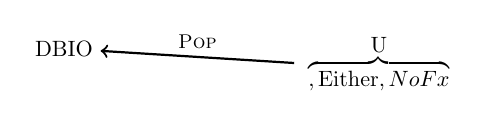
\begin{tikzpicture}[scale=0.8, every node/.style={scale=0.8}]
        \node (A) at (0, 0) [above] {%
          $\overbrace{\SThree{ ,\lstinline|Either|,NoFx}}^{\lstinline|U|}$
        };
        \node (B) at (-5, 0.55) [above] {\lstinline|DBIO|};   
        \draw [thick, ->] ($ (A.west) + (-0.1, 0) $) -- (B) node[pos=0.5, above] {%
          {\small\textsc{Pop}}
        };
      \end{tikzpicture}
    \end{center}

    \item<+-> An interpreter provides two values for us:
    \begin{enumerate}
      \item \lstinline|DBIO[X]|
      \item continuation: \lstinline|X => Eff[U, B]|
    \end{enumerate}
    to implement the monad instace for the effect
    
    \begin{itemize}
      \item So we define \lstinline|map| and \lstinline|flatMap|
      from the two parts
    \end{itemize}
  \end{itemize}

  \uncover<+->{%
    \simplecallout[\LARGE\ce{:thinking:}]{-}{green!10}{%
      What is continuation?
    }%
  }

  \begin{notes}
    \item いま、\lstinline|DBIO|のインタープリターを\lstinline|Eff[R, A]|、
    ただし\lstinline|R|は$\SThree{\lstinline|DBIO|,\lstinline|Either|,NoFx}$という
    状況について考えていく。

    \item 図のように\lstinline|R|から\lstinline|DBIO|が取り出される。
    ここで残ったエフェクトスタックを\lstinline|U|と呼び
    $\STwo{\lstinline|Either|,NoFx}$である。

    \item このとき、インタープリターはモナドインスタンスの実装のために
    次の2つを提供してくれる。この例でいえば、これらを使って我々はモナドインスタンスの
    ための\lstinline|map|と\lstinline|flatMap|をあたえなければならない。

    \item ところで、ここでいう\ballcircle{2}の継続(\emph{continuation})とは
    いったいどういうことだろうか?
  \end{notes}
\end{frame}

\begin{frame}
  \frametitle{Notation}

  \begin{itemize}
    \item First, we introduce a new notation to \lstinline|R|
    before explain
    
    \item Assuming that \lstinline|R: _dbio: _either|, it means
    \lstinline|R| is $\SThree{\lstinline|DBIO|,\lstinline|Either|,NoFx}$
  \end{itemize}

  \begin{notes}
    \item 説明のまえに、エフェクトスタックをのための新しい表記を導入する。

    \item いま\lstinline|R: _dbio: _either|と書いたら、これは
    \lstinline|R|が$\SThree{\lstinline|DBIO|,\lstinline|Either|,NoFx}$という
    エフェクトスタックであることを意味する。
    このようにすると\lstinline|Eff[R: _either, A]|などと書けて便利である。
  \end{notes}
\end{frame}

\begin{frame}
  \frametitle{Continuation for interpreter}

  \begin{itemize}
    \item<+-> There are some \lstinline|DBIO| operations in the \lstinline|Eff[R: _dbio: _either, A]|
    
    \begin{center}
      \begin{tikzpicture}[scale=0.7, every node/.style={transform shape}]
        \node (A) at (0, 0) [above, align=center] {%
          {
\includegraphics[width=0.05\textwidth]{./img/ai_computer_sousa_robot.png}} \\
          Interpreter for \lstinline|DBIO|
        };

        \node (B) at (6, -1.5) [above, align=center] {%
          {
\includegraphics[width=0.05\textwidth]{./img/ai_computer_sousa_robot.png}} \\
          Interpreter for \lstinline|DBIO|
        };

        \node (C) at (-2.5, -1) [left] {%
          \lstinline|Eff[R: _dbio: _either, A]|
        };

        \node (D) at (7, -2.5) [right] {$\cdots$};
        \node (E) at (7, -3.5) [right] {$\cdots$};

        \node (F) at (-2.5, -5) [left] {%
          \lstinline|Eff[R: _either, DBIO[A]]|
        };
        
        \draw [thick, -] (A) -- (0, -5.2);
        \draw [thick, -] (B) -- (6, -4.7);
        \draw [thick, ->] (C.east) -- (0, -1);

        \draw [thick, ->] (0, -2) -- (6, -2);
        \draw [thick, ->] (6, -2.5) -- (D);
        \draw [thick, ->] (E) -- (6, -3.5);
        \draw [thick, ->] (6, -4) -- (0, -4);
        \draw [thick, ->] (0, -5) -- (F);

        \node [rectangle, fit={(3.5, 0) (8.5, -4.5)}, inner sep=0pt, thick, draw=red!90] (G) {};
        \node (H) at (4, -6) [above] {%
          \textbf{Continuation}
        };
        \draw [ultra thick, ->] (H) -- (G);
      \end{tikzpicture}
    \end{center}

    \item<+-> First interpreter can access the continuation as a function,
    which processes effect recursivily
  \end{itemize}

  \begin{notes}
    \item このように合成されたインタープリターが処理するときには、
    現在処理しているモナドよりも後の部分を継続として得ることができる。

    \item そして全ての処理が終了するとエフェクトが実際に発生して、
    エフェクトスタックにあった型が結果側へ移動する。
  \end{notes}
\end{frame}

\begin{frame}
  \frametitle{Extract types by interpreter}

  \pause
  \begin{itemize}
    \item<+-> \emph{Some} types in the effects stack \lstinline|R| can be
    extracted by \emph{one} interpreter
    \begin{center}
      \begin{tikzpicture} %[scale=0.8, every node/.style={scale=0.8}]
        \node (A) at (0, 0) [right] {%
          $\SThree{ , ,NoFx}$
        };
        \node (B) at (-4, 0) [left] {\lstinline|DBIO[Either]|};
        \node (C) at (-2, -1.6) [above] {
          {
\includegraphics[width=0.1\textwidth]{./img/ai_computer_sousa_robot.png}}
        };
        \draw [thick, ->] ($ (A.west) + (-0.1, 0) $) -- (B) node[pos=0.5, above] {%
          {\small\textsc{Pop}}
        };
      \end{tikzpicture}
    \end{center}

    \item<+-> On the other hand, it's good\ce{:person_gesturing_ok:} that an interpreter doesn't extract just any types from the effects stack
    \begin{center}
      \begin{tikzpicture} %[scale=0.8, every node/.style={scale=0.8}]
        \node (A) at (0, 0) [right] {%
          $\SThree{\lstinline|DBIO|,\lstinline|Either|,NoFx}$
        };
        \node (B) at (-6, 0) [left] {$Void$};
        \calloutquote[
          at={(-3, -0.5)},
          width=4.1cm,
          position={(0.1,-0.2)},
          author={
\includegraphics[width=0.1\textwidth]{./img/ai_computer_sousa_robot.png}},
          fill=cyan!10
        ]{\footnotesize
          But I will do something...
        };
        \draw [thick, ->] ($ (A.west) + (-0.1, 0) $) -- (B);
      \end{tikzpicture}
    \end{center}
  \end{itemize}

  \begin{notes}
    \item また、これまでの例では1つのインタープリターが1つの型を
    エフェクトスタックから取り出して処理をするという説明をしてきたが、
    実はこのように2つ以上の型を1つのインタープリターで同時に処理してもよい。

    \item さらに0個処理する、つまりはエフェクトスタックから何も取り除かないような
    インタープリターもOKである。
  \end{notes}
\end{frame}

\section{Interpreter Handling over Effects}

\begin{frame}
  \frametitle{Table of contents}
  \tableofcontents[currentsection]

  \begin{notes}
    \item さて、ここまででEffとそのインタープリターの紹介が終ったので、
    ここからはさきほどまで見てきた具体的な問題である「DBアクセスとメール送信」の
    話題に戻っていく。
  \end{notes}
\end{frame}

\begin{frame}
  \frametitle{Revisit the problem}

  \begin{itemize}
    \item<+-> We want to take the both cohesion and consistency between
    the database transaction and sending e-mails

    \item<+-> ``Over effects'' means that
    \begin{itemize}
      \item There are two effects: the database I/O and sending e-mails

      \item If database I/O with trasaction would fail,
      sending e-mails must \emph{not} be done

      \item What an effect should be run
      depends on that the other effect would be done successfully or not
    \end{itemize}
  \end{itemize}

  \begin{notes}
    \item 我々はメール送信とデータベースのトランザクションにおける
    凝集度と一貫性の両方を達成したい。

    \item タイトルにある``over effects''とはこのように
    2つのエフェクトが相互に関係して「片方が成功したらもう片方をやる」
    といったことを記述することを意図している。
  \end{notes}
\end{frame}

\begin{frame}[fragile]
  \frametitle{Create a type constructor}

  \begin{itemize}
    \item First we make a type constructor for e-mail
    \begin{columns}
      \begin{column}{0.45\textwidth}
\begin{lstlisting}[style=scala]
sealed trait MailAction[A]
case class Tell(
  mail: Mail
) extends MailAction[Unit]
\end{lstlisting}
      \end{column}
      \begin{column}{0.55\textwidth}
        \simplecallout[\Large\ce{:thinking:}]{-}{cyan!10}{%
          This is just like \lstinline|Writer| monad, isn't it?
        }
      \end{column}
    \end{columns}

    \item And we define \lstinline|DBIOAction| too
    \begin{columns}
      \begin{column}{0.45\textwidth}
\begin{lstlisting}[style=scala]
sealed trait DBIOAction[A]
case class Ask() extends DBIOAction[Session]
case class Execute[A](
  value: A
) extends DBIOAction[A]
\end{lstlisting}
      \end{column}
      \begin{column}{0.55\textwidth}
        \simplecallout[\Large\ce{:face_with_monocle:}]{+}{green!10}{%
          It's like \lstinline|Reader| moand, the same as \lstinline|DBIO|
        }
      \end{column}
    \end{columns}
  \end{itemize}

  \begin{notes}
    \item まずメールを\lstinline|Eff|のエフェクトスタックに載せるために
    このような型コンストラクター\lstinline|MailAction|を作っておく。

    \item sealed traitになっていて、唯一の値として\lstinline|Tell|を持つ。
    これは中身に\lstinline|Mail|な値を持つ。

    \item これが\lstinline|Writer|モナドに見える(?)かもしれないが、
    それの理由は後に解説する。

    
    \item 次に\lstinline|DBIOAction|というDB用の型を定義する。
    \lstinline|DBIO|がほぼ\lstinline|Reader|モナドであったように、
    Effでも似たような構造になる。
  \end{notes}
\end{frame}

\begin{frame}[fragile]
  \frametitle{Utilty functions}

  \begin{itemize}
    \item Then we create utilty functions:
    \begin{enumerate}
      \item First one \lstinline|sendMailEff| is
    for making \lstinline|Eff[R: _mail, Unit]|
\begin{lstlisting}[style=scala]
def sendMailEff[R: _mail](
  mail: Mail
): Eff[R, Unit] = Eff.send[MailAction, R, Unit](Tell(mail))
\end{lstlisting}

      \item Second one \lstinline|fromDBIO| is
      used to convert \lstinline|DBIO[A]| into \lstinline|Eff[R: _dbio, A]|

\begin{lstlisting}[style=scala]
def fromDBIO[R: _dbio, A](
  dbio: DBIO[A]
): Eff[R, A] =
  for {
    session <- Eff.send[DBIOAction, R, Session](Ask())
    a <- Eff.send[DBIOAction, R, A](Execute(dbio.run(session)))
  } yield a
\end{lstlisting}
    \end{enumerate}
  \end{itemize}

  \begin{notes}
    \item まずは\lstinline|Eff[R: _mail, Unit]|を作成するための
    \lstinline|sendMailEff|と既存の\lstinline|DBIO[A]|を\lstinline|Eff[R: _dbio, A]|
    へと変換する関数\lstinline|fromDBIO|を作成する。

    \item これらはatnos-effで定義されている\lstinline|Eff.send|を使って実装する。
    \begin{itemize}
      \item この\lstinline|Eff.send|をきちんとコードで追うためには、
      さきほど説明した\lstinline|Eff|のエフェクトスタックが実際にどう表現されているのか?
      ということを詳細に理解する必要があるため、いったんここではあえて説明しない。

      \item とりあえずのところは、型コンストラクターに包まれたような\lstinline|M[A]|において、
      この\lstinline|M|をエフェクトスタックへ適切に追加してくれるものという理解でよいと思う。
    \end{itemize}

    \item \lstinline|DBIO[A]|から\lstinline|Eff[R: _dbio, A]|を作るのは少し大変となる。

    
    \item まずは\lstinline|Ask|を使って\lstinline|Eff[R: _dbio, Session]|をとする。
    そして\lstinline|for|の中でまわすことで\lstinline|session: Session|を得る。
    これで\lstinline|dbio.run(session)|を\lstinline|Execute|の中で行なえば
    狙った型にすることができる。    
  \end{notes}
\end{frame}

\begin{frame}[fragile]
  \frametitle{Type parameters in interpreter}

  \begin{itemize}
    \item We have already seen, \lstinline|Interpreter| (page \ref{fra:interface_interpreter})
    has such a type parametrs:
\begin{lstlisting}[style=scala]
trait Interpreter[M[_], R, A, B]
\end{lstlisting}
    which mean that\ce{:point_down:}
  \end{itemize}

  \begin{columns}
    \begin{column}{0.6\textwidth}
      \begin{center}
        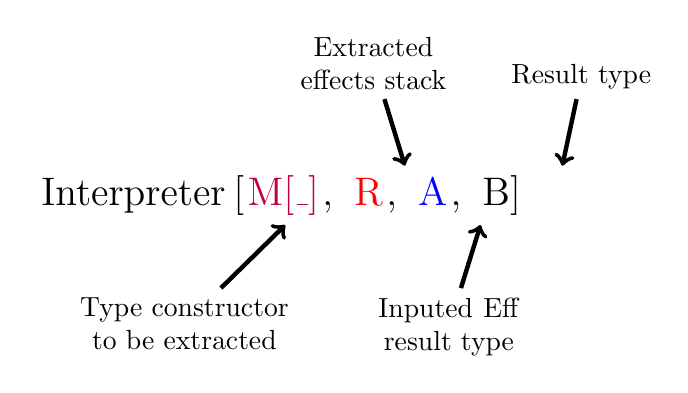
\begin{tikzpicture}[scale=0.8]
          \node (A) at (0, 0) [above] {\Large
            \lstinline|Interpreter[|%
            \textcolor{purple}{\lstinline|M[_]|}\lstinline|, |%
            \textcolor{red}{\lstinline|R|}\lstinline|, |%
            \textcolor{blue}{\lstinline|A|}\lstinline|, |%
            \lstinline|B]|%
          };
       
          \node (B) at (-1.5, -1) [below, align=center] {%
            Type constructor \\
            to be extracted%
          };
       
          \node (C) at (1.5, 2) [above, align=center] {%
            Extracted \\
            effects stack%
          };
       
          \node (D) at (2.7, -1) [below, align=center]{%
            Inputed \lstinline|Eff| \\
            result type%
          };
       
          \node (E) at (4.8, 2) [above]{%
            Result type%
          };
       
          \draw [ultra thick, ->] (B) -- ($ (A.south) + (0.1, 0) $);
          \draw [ultra thick, ->] (C) -- ($ (A.north) + (2, 0) $);
          \draw [ultra thick, ->] (D) -- ($ (A.south) + (3.2, 0) $);
          \draw [ultra thick, ->] (E) -- ($ (A.north) + (4.5, 0) $);
        \end{tikzpicture}
      \end{center}   
    \end{column}
    \begin{column}{0.4\textwidth}
      \pause
      \simplecallout[%
        {
\includegraphics[width=0.2\textwidth]{./img/computer_man.png}}%
      ]{+}{yellow!10}{%
        It's very complicated\ce{:innocent:}\\
        I want to see examples!
      }
    \end{column}
  \end{columns}

  \begin{notes}
    \item ここでは先程みた\lstinline|Interperter|の各型パラメーターについて説明していく。

    \item この図の通りになっているが、複雑というかイメージが掴みにくいかもしれないので
    さっそく例を見ていく。
  \end{notes}
\end{frame}

\begin{frame}
  \frametitle{Example}

  \begin{center}
    \begin{tikzpicture}
      \node (A) at (0, 1) [above] {%
        \lstinline|Eff[R: _dbio: _mail, A]|
      };
      
      \node (B) at (0, -2) [above, align=center] {%
        {
\includegraphics[width=0.1\textwidth]{./img/ai_computer_sousa_robot.png}} \\
        \lstinline|Interpreter[DBIOAction, U, A, Either[Throwable, A]]|     
      };

      \node (C) at (0, -3.5) [above] {%
        \lstinline|Eff[R: _mail, Either[Throwable, A]]|
      };

      \draw [thick, ->] (A) -- (B);
      \draw [thick, ->] (B) -- (C);
    \end{tikzpicture}
  \end{center}

  \begin{itemize}
    \item Note that \lstinline|R: _mail| means \lstinline|MailAction| is
    contained in the effects stack \lstinline|R|

    \item And \lstinline|U| is $\STwo{\lstinline|Mail|,NoFx}$.
    We can calculate \lstinline|U| from \lstinline|R| and \lstinline|DBIOAction|
    by \lstinline|Member.Aux[DBIOAction, R, U]|
  \end{itemize}

  \begin{notes}
    \item このようにまず\lstinline|R|が$\SThree{\lstinline|DBIOAction|,\lstinline|Mail|,NoFx}$という
    \lstinline|Eff[R: _dbio: _mail, A]|が、このように型パラメーターを入れた
    インタープリターに入力するとする。

    \item すると図の下にあるような型の\lstinline|Eff|となる。

    \item また、エフェクトスタック\lstinline|R|から\lstinline|DBIOAction|を取り除いた
    残りのエフェクトスタックは\lstinline|Member.Aux[DBIOAction, R, U]|という
    型クラス(\emph{type class})によって型\lstinline|U|で得られる。
  \end{notes}
\end{frame}

\begin{frame}[fragile]
  \label{fra:define_runDBIO}
  \frametitle{Implement the interpreter}

  \pause
  \begin{itemize}
    \item<+-> It's time to implement the interpreter over
    effects!

    \item<+-> We'll make \lstinline|DBIOAction| interpreter
    at first

    \item<+-> It means that we implement
    \lstinline|Interpreter[DBIOAction, U, A, Either[Throwable, A]]| for
    \lstinline|Eff[R: _dbio, A]|
    \begin{itemize}
      \item \lstinline|U| is the rest of \lstinline|DBIOAction| extracted from \lstinline|R|
    \end{itemize}

    \item<+-> Finally \lstinline|runDBIO| has this interface:
\begin{lstlisting}[style=scala]
def runDBIO[R: _dbio, A](
  eff: Eff[R, A]
)(implicit m: Member.Aux[DBIOAction, R, NoFx]): Either[Throwable, A] =
  withTransaction { session =>
    Eff.run(
      Interpret.runInterpreter(eff)(new Interpreter[DBIOAction, NoFx, A, Either[Throwable, A]] {
        /* We implement now! */
      })
    )
  }
\end{lstlisting}
  \end{itemize}

  \begin{notes}
    \item ここからいよいよインタープリターを実装していく。
    まず\lstinline|DBIOAction|のインタープリターを実装する。

    \item 下のコードを見てほしいが、このインタープリターは
    \lstinline|Member.Aux[DBIOAction, R, NoFx]|のインスタンスを取ることによって
    エフェクトスタックが\lstinline|DBIOAction|しかない状態を強制している。
    エフェクトスタックが空($NoFx$)のとき、\lstinline|Eff.run|によって
    \lstinline|Eff[R, A]|の\lstinline|A|を取得できる。

    \item そして、このようにインタープリターの定義を全部
    ローンパターンのときに作った\lstinline|withTransaction|の中に押し込んでいる。
    これは後で重要になるが、これによってインタープリター内部で\lstinline|session|にアクセスできるようになる。
  \end{notes}
\end{frame}

\begin{frame}[fragile]
  \frametitle{1st: \lstinline|onPure|}

  \begin{itemize}
    \item<+-> Following \lstinline|Interpreter| interface in page \ref{fra:interface_interpreter},
    we make \lstinline|onPure| at first
\begin{lstlisting}[style=scala]
def onPure(a: A): Eff[NoFx, Either[Throwable, A]] =
  Eff.pure(Right(a))
\end{lstlisting}

    \item<+-> It's very easy\ce{:upside_down:}
  \end{itemize}

  \begin{notes}
    \item このページのインターフェースにしたがって、
    まずは\lstinline|onPure|をつくっていく。
    といってもこれはモナドの\lstinline|pure|が簡単なように
    すごく簡単に作ることができる。
  \end{notes}
\end{frame}

\begin{frame}[fragile]
  \frametitle{2nd: \lstinline|onEffect|}

  \begin{itemize}
    \item Next we implement \lstinline|onEffect|

    \pause
\begin{lstlisting}[style=scala]
def onEffect[X](
  x: DBIOAction[X], continuation: Continuation[NoFx, X, Either[Throwable, A]]
): Eff[NoFx, Either[Throwable, A]] =
  x match {
    case Ask() => continuation(session)
    case Execute(v) => continuation(v)
  }
\end{lstlisting}

    \begin{itemize}
      \item \lstinline|Continuation[U, X, Either[Throwable, A]]| reperesents
      a function whose interface is \lstinline|X => Eff[U, Either[Throwable, A]]|
    \end{itemize}

    \pause
    \item First we have to use the pattern matching for \lstinline|x|
    to determine what \lstinline|X| is
    \begin{description}
      \item[\texttt{Ask} case] \lstinline|X| is \lstinline|Session|,
      and \lstinline|continuation| is needed that value

      \item[\texttt{Execute} case] we don't know what \lstinline|X| is,
      but \lstinline|Execute| has \lstinline|X| value\ce{:+1:}
    \end{description}

    \pause
    \item We can access \lstinline|session| because
    the interpreter is in \lstinline|withTransaction| (page \ref{fra:define_runDBIO})
  \end{itemize}

  \begin{notes}
    \item 次は\lstinline|onEffect|である。
    このケースでは\lstinline|x: DBIOAction[X]|に対してパターンマッチをする。

    \item
    \begin{description}
      \item[\texttt{Ask}のとき]
      外にある\lstinline|withTransaction|で
      捕獲しておいた\lstinline|session|があるので、それを\lstinline|continuation|に
      いれることで継続を実行できる

      \item[\texttt{Execute}のとき]
      \lstinline|Execute|が持つ\lstinline|X|の値を使って継続を実行できる
    \end{description}    

    \item そして\lstinline|Continuation[U, X, Either[Throwable, A]]|は
    \lstinline|X => Eff[U, Either[Throwable, A]]|みたいな関数のインターフェースを継承しているので、
    ここに上で得た\lstinline|X|型の値を入れてることで\lstinline|onEffect|の返り値と
    同じ型を得ることができる。
  \end{notes}
\end{frame}

\begin{frame}[fragile]
  \frametitle{3rd: \lstinline|onLastEffect| and \lstinline|onApplicativeEffect|}

  \begin{itemize}
    \item<+-> These are just type puzzle
\begin{lstlisting}[style=scala]
def onLastEffect[X](x: DBIOAction[X], continuation: Continuation[NoFx, X, Unit]): Eff[NoFx, Unit] =
  x match {
    case Ask() => continuation(session)
    case Execute(v) => continuation(v)
  }
  
def onApplicativeEffect[X, T[_]: Traverse](
  xs: T[DBIOAction[X]], continuation: Continuation[NoFx, T[X], Either[Throwable, A]]
): Eff[NoFx, Either[Throwable, A]] =
  continuation.apply(
    xs.map {
      case Ask() => session
      case Execute(v) => v
    }
  )
\end{lstlisting}

    \item<+-> I know that it's very diffcult for us
    but applicative interpreter is not the scope in this talk
    so we'll skip
  \end{itemize}

  \begin{notes}
    \item ここはatons-effの\lstinline|Interpreter|のインターフェース上
    必要なので作っただけという側面が強い。おそらくアプリカティブのときには
    \lstinline|Future|を並列にするとかそういうパフォーマンスの向上のためにある気がする。

    \item そういう理由なので、いったんこれの説明は割愛する。
  \end{notes}
\end{frame}

\begin{frame}
  \frametitle{Interpreter for \lstinline|MailAction|}

  \pause
  \begin{itemize}
    \item<+-> We have already gotten the interpreter for \lstinline|DBIOAction|
    so then we'll create a new interpreter for \lstinline|MailAction|

    \item<+-> The interface is
    \lstinline|Interpreter[MailAction, U, A, (List[Mail], A)]| for
    \lstinline|Eff[R: _mail, A]|
    \simplecallout[%
      {
\includegraphics[width=0.1\textwidth]{./img/computer_man.png}}%
    ]{+}{yellow!10}{%
      What is \lstinline|(List[Mail], A)|?   
    }

    \item<+-> We try to
    \begin{enumerate}
      \item \label{enum:collect_email}
      collect e-mails by a new interpreter we'll create from now

      \item execute \lstinline|runDBIO| then if the result is successful
      run \lstinline|sendMail| with \ballref{enum:collect_email}'s e-mails.
      However if the result is failure \lstinline|sendMail| is not call
      and \ballref{enum:collect_email}'s e-mails will not be sent
    \end{enumerate}
  \end{itemize}

  
  \begin{notes}
    \item そういうわけで\lstinline|DBIOAction|のインタープリターが完成したので
    つぎにメールのやつをつくる。

    \item 定義時にも述べたように、これのインタープリターはこのように結果の型が
    \lstinline|Writer|モナドのタプルのようになっている。

    \item これはどういうことかというと
    いったんはこのように送信するメールを\lstinline|List[Mail]|として
    蓄えておいて、そしてそのあとで\lstinline|runDBIO|を実行して
    それが成功していた場合はそのリストの内容を全て送信処理に回すという作戦である。

    \item もしデータベース処理で失敗がおきていれば、メールのリストは破棄して
    メールを送信しない。
  \end{notes}
\end{frame}

\begin{frame}[fragile]
  \frametitle{Interpreter for \lstinline|MailAction|}

  \begin{itemize}
    \item So \lstinline|sendMailAfterDBIO|'s interface:
\begin{lstlisting}[style=scala]
def runMailAfterDBIO[R: _mail: _dbio, U, A](
  eff: Eff[R, A]
)(
  implicit m1: Member.Aux[MailAction, R, U], m2: Member.Aux[DBIOAction, U, NoFx]
): Either[Throwable, A] = {
  val mailRemoved: Eff[U, (List[Mail], A)] =
    Interpret.runInterpreter(eff)(new Interpreter[MailAction, U, A, (List[Mail], A)] {
      /* We implement now! */
    })

  runDBIO(mailRemoved).flatMap {
    case (mails, a) => 
      mails.traverse(sendMail).map(_ => a)
  }
}
\end{lstlisting}

    \begin{itemize}
      \item Note that \lstinline|sendMail| is defined on \ref{fra:send_email_definition} page
    \end{itemize}
  \end{itemize}

  \begin{notes}
    \item そういうわけでDB処理を実行して
    成功していたらメールを送る関数\lstinline|runMailAfterDBIO|はこのようになる。

    \item 内部で\lstinline|runDBIO|を使う関係で、これもエフェクトスタックが
    ちょうど$\SThree{\lstinline|MailAction|,\lstinline|DBIOAction|,NoFx}$であるように
    \lstinline|Member.Aux|で調整している。

    \item まずはこれから作るメール用のインタープリターでメールと結果を分離してタプルにする。
    そのあとで\lstinline|runDBIO|の結果をみて実際にメールを送信する\lstinline|sendMail|
    を呼ぶかどうか?を決定する。
  \end{notes}
\end{frame}

\begin{frame}[fragile]
  \frametitle{Interpreter for \lstinline|MailAction|}

  \begin{itemize}
    \item This is it!
\begin{lstlisting}[style=scala]
trait Interpreter[MailAction, U, A, (List[Mail], A)] {
  def onPure(a: A): Eff[U, (List[Mail], A)] =
    Eff.pure((Nil, a))

  def onEffect[X](
    x: MailAction[X], continuation: Continuation[U, X, (List[Mail], A)]
  ): Eff[U, (List[Mail], A)] =
    x match {
      case Tell(mail) =>
        // `Tell extends MailAction[Unit]` so in this case `X` is `Unit`
        continuation(()).map {
          case (mails, a) => (mail :: mails, a)
        }
    }
}
\end{lstlisting}
    \begin{itemize}
      \item \lstinline|onLastEffect| and \lstinline|onApplicativeEffect|
      are omited from the slide\ce{:innocent:}
    \end{itemize}
  \end{itemize}

  \begin{notes}
    \item そしてインタープリターがこれ!

    \item \lstinline|onEffect|のところで、いま\lstinline|MailAction|は
    型パラメーターとして任意の型を取ることができる。しかし唯一の値である\lstinline|Tell|は
    \lstinline|MailAction[Unit]|で固定されているため、
    したがってここに来た時点で\lstinline|X|は\lstinline|Unit|ということになる。
    あとは継続を呼び出しつつメールをリストに追加するだけである。
    \begin{itemize}
      \item ここでは\lstinline|Tell|しかパターンがないものの、\lstinline|X|が
      \lstinline|Unit|であることをコンパイラーに教えるためにパターンマッチをしておく。
    \end{itemize}

    \item さきほどの理由があって\lstinline|onLastEffect|と\lstinline|onApplicativeEffect|は
    省略する。
  \end{notes}
\end{frame}

\begin{frame}[fragile]
  \frametitle{Usage}

  \begin{itemize}
    \item<+-> We can use this like below:
\begin{lstlisting}[style=scala]
def userUpdateEff[R: _dbio: _mail](
  newUserInfo: UserInfo
): Eff[R, Unit] =
  for {
    _ <- fromDBIO(userUpdate(newUserInfo))
    _ <- sendMailEff(Mail(/* very great email from `newUserInfo`*/))
  } yield ()
\end{lstlisting}

\begin{lstlisting}[style=scala]
val user: UserInfo = ???

runMailAfterDBIO(userUpdateEff(user)) match {
  case Right(_) => /* Succecss DB and e-mail! */
  case Left(_)  => /* Failure */
}
\end{lstlisting}

    \item<+-> It looks good, doesn't it?\ce{:thinking}
  \end{itemize}

  \begin{notes}
    \item さて、実際完成したインタープリターなどはこのように使うことができる。
    \lstinline|userUpdateEff|は見てのとおり、ユーザーのアップデート処理のすぐあとに
    メール送信処理が書いてあり、見通しがよいと思われる。
  \end{notes}
\end{frame}

\section{Conclusion}

\begin{frame}
  \frametitle{Discussion: Monad vs Eff}

  \pause
  \uncover<+->{%
    \simplecallout[%
      {
\includegraphics[width=0.1\textwidth]{./img/computer_man.png}}%
    ]{-}{red!10}{%
      This example can be done by monad (transformer)?
    }%
  }%

  \begin{itemize}
    \item<+-> That's correct, but
    \begin{itemize}
      \item in this example only covers a case in which,
      ``if the transaction fails no e-mail is sent''

      \item other cases could exist;
      for example, maybe we would like to send error e-mails
      when the transaction fails
    \end{itemize}

    \item<+-> If we do that with monads,
    we cannot make it without changing interfaces to distinguish
    whether an e-mail will be sent or not when a transaction fails

    \item<+-> Eff can do that without changing any interfaces,
    we only change the interperter.\footnote[frame]{%
      but I cannot explain this due to the time limit of this talk\ce{:innocent:}
    }%
  \end{itemize}

  \begin{notes}
    \item ここまでの例を見て、これはモナドやモナドトランスフォーマー
    でも達成できたのでは?というふうに思うかもしれない。

    \item 実はこの例だけだとそういうことになるが、たとえばさらに複雑にする方法として
    \begin{itemize}
      \item 今回はトランザクションが失敗したらメールは全て破棄という方針であったが、
      実際にはエラーメッセージの送信など一部のメールは送るという場合もある。

      \item そういうときにモナドトランスフォーマーのアプローチは型(インターフェース)を変更して
      「失敗したときに破棄するところ」と「失敗したら送るところ」を分ける必要があると思う。
    \end{itemize}

    \item 一方でEffはそのような変更なしで特定の部分の変更をなかったことにする(継続を適用しない)
    といったことがインターフェースの変更なしで達成できる。
    \begin{itemize}
      \item ちょっと時間がないのでここでは説明しないけど……。
    \end{itemize}
  \end{notes}
\end{frame}

\begin{frame}[fragile]
  \frametitle{Discussion: Monad vs Eff}

  \begin{itemize}
    \item<+-> Or, we can call \lstinline|sendMail| outside
    of monads
\begin{lstlisting}[style=scala]
val dbioMail: Writer[List[Mail], DBIO[?]] = ???

val (mails, dbio) = dbioMail.run // `Writer` run
withTransaction(dbio.run) match {
  case Right(_) => List.traverse(mails)(sendMail)
  case Left(_)  => // error!
}
\end{lstlisting}

    \item<+-> Indeed it can be done but it's outside of monad,
    so it's maybe not succesful to reprensenting effects by monad\ce{:thinking:}
  \end{itemize}

  \begin{notes}
    \item このようにモナドの外側に処理を書くことで、失敗したときにもメールを送るか
    送らないか、を制御できることはできる。

    \item たしかにこれで達成できてはいるが、これはあくまでモナドの外側で行なわれたことであり、
    つまり作用(エフェクト)をモナドで表現するということに完全に成功しているのか?
    というと個人的には疑問が残る。
  \end{notes}
\end{frame}

\begin{frame}
  \frametitle{Conclusion}

  \pause
  \begin{itemize}
    \item<+-> In this talk,
    we see that some ways to database I/O and sending e-mails

    \item<+-> Monad types are embedded its concrete operation for the effect
    but Eff is not. Types are just symbols and the concrete operation is given
    by the interpreter

    \item<+-> Therefore an interpreter can do the complex operation
    which is over some effects
    
    \item<+-> Let's use Eff!
  \end{itemize}

  \begin{notes}
    \item というわけで、このトークではデータベースI/Oのいろいろなやり方を紹介した。

    \item モナドはその型自体に具体的なエフェクトのためのオペレーションが記述されているが、
    一方でEffの場合、型は単なるシンボルであって実際の操作はインタープリターが持っている。

    \item それによって複数のエフェクトを跨ぐような複雑な操作を行うことができる。

    \item Effを使っていこう!
  \end{notes}
\end{frame}

\section*{References}

\begin{frame}%[allowframebreaks]
  \frametitle{References}

  \nocite{*}
  \bibliographystyle{junsrt_url}
  \bibliography{ref}

  \begin{notes}
    \item この資料はOlegさんと論文と同名だが、
    Eff論文の共著者である石井さん日本語による解説発表となっている。

    \item ScalaMatsuriには日本人の方が多いと思うので、
    ソースコードはHaskellとなってはいるが、この資料がとても参考になると思う。

    \item このスライドを執筆するときにもおおいに参考になった。
  \end{notes}
\end{frame}

\begin{frame}
  \centering
  {\Huge Thank you for your attention!}
\end{frame}

\end{document}
